\documentclass{thesis-ekf}
\usepackage[T1]{fontenc}
\usepackage{amsthm,fancyhdr,mathtools,amssymb,listingsutf8,xcolor}
\PassOptionsToPackage{defaults=hu-min}{magyar.ldf}
\usepackage[magyar]{babel}
\lstset{
inputencoding=utf8/latin2,
language=HTML,
numbers=left,
xleftmargin=2cm,
xrightmargin=2cm,
breaklines,
postbreak=\hbox{$\color{red}\hookrightarrow\ $},
backgroundcolor=\color{gray!30},
frame=tblr,
framesep=3pt,
keywordstyle=\bfseries\color{blue},
commentstyle=\itshape\color{teal}
}
\footnotestyle{rule=fourth}
\DeclareMathOperator{\tg}{tg}
\theoremstyle{definition}
\newtheorem{definicio}{Definíció}[chapter]
\begin{document}
	\institute{Matematikai és Informatikai Intézet}
	\title{2. feladat}
	\author{Eperjesi Attila Dávid\\Programtervező informatikus BSc}
	\supervisor{Tómács Tibor\\egyetemi docens}
	\city{Eger}
	\date{2020}

	\maketitle
	\tableofcontents
	\chapter{Az alapok}
	\section{A web és a látogató viszonya}
	Webfejlesztőként magunk is látogatók vagyunk. Nap mint nap különböző weboldalakat látogatunk meg. Ahhoz azonban, hogy jó weboldalakat tudjunk készíteni, olyan módon kell látnunk a weboldalakat, ahogy azt korábban nem tettük. Folyamatosan szem előtt kell tartanunk mérnöki szempontokat is.
	\subsection{Webes tipográfiai alapismeretek}
	Sokunkkal próbálták jól-rosszul megtanítani a szövegszerkesztési alapismereteket. Azonban a papíralapú szövegszerkesztéssel kapcsolatos tanulmányaink hátrányunkra válhatnak, ha nem értjük meg a papír és a weboldal mint különböző médiák közötti különbségeket.
	
	A nyomdászoknak sokféle lehetőség áll a rendelkezésükre, amikor szóba kerül a tipográfia, mint például a betűkészletek puszta száma vagy az elrendezési lehetőségek széles skálája. A webes tipográfia ennél sokkal korlátozottabb, mivel olyan típusokkal és elrendezéssel kell dolgozzunk, amelyről tudjuk, hogy elérhető és használható lesz azokon a gépeken is, amelyeken az olvasók megnyitják a lapot, hiszen senki nem fejleszt saját magának weboldalt.\footnote{Paul Haine: Tipográfia a weben című cikke alapján}
	\subsection{Hogyan olvasunk a weben?}
	Ha weboldal készítésére adjuk fejünket, akkor jó, ha tisztában vagyunk a látogatói szokásokkal. E témát egyre többen és egyre árfogóbban kutatják. Itt most csak egy rövid ajánló erejéig foglalkozunk a témával. Legalább a következő cikkek elolvasása célszerű a továbbhaladás előtt:
	\begin{itemize}
		\item Kámán Veronika: A jelen forradalma: olvasás weben
		\item Kovács Balázs: Írás és olvasás a weben
	\end{itemize}
	\subsection{Kereső(re) optimalizálás}
	Ha egy weboldalt fáradságos munkával elkészítettünk, szeretnénk, ha minél több látogató magtalálná az oldalunkat. Aki elolvassa a cikkeinket, hozzászól a blogunkhoz, vásárol a termékeink közül.
	
	A látogató ,,szerzése'' minden honlapnak célja. A látogatószerzés klasszikus módja a keresőmotorokban (pl. Google) való megjelenés, mégpedig minél előkelőbb helyen az általunk hőn áhított keresőszavakra. Bár a témával foglalkozó írások, weboldalak, vállalkozások nem mindig tesznek különbséget a keresőoptimalizálás és keresőmarketing között, itt ezt megtesszük.
	\begin{itemize}
		\item A keresőre optimalizálás a saját oldalunk fejlesztésével történik. Emiatt minden weboldal-tulajdonosnak szüksége van rá. Mi itt erre tudunk koncentrálni.
		\item A keresőmarketing sok egyéb eszközt (pl. Hírlevél, fizetett hirdetések) is felhasznál, amelyek nem képezik a weboldalunk részét. (Ez a terület nem témája a könyvnek.)
	\end{itemize}
\section{A web működése}
\Az{\ref{fig:kliensszerver}}.~ábra sokat segíthet a további információk megértésében.
\begin{figure}[th!]
	\centering
	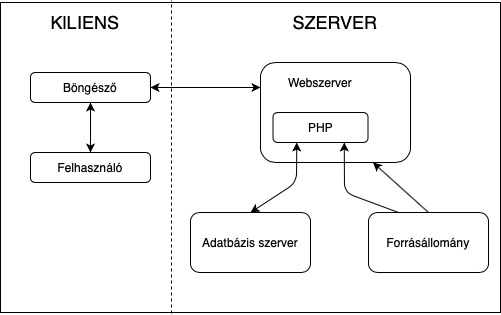
\includegraphics[width=5cm]{kliensszerver}
	\caption{A kliens-szerver architektúra}
	\label{fig:kliensszerver}
\end{figure}

A  \emph{felhasználó}, aki a web szolgáltatásait ki akarja használni, megteheti ezt egy tetszőleges modern \emph{webböngészővel}. (E két  \emph{,,szereplő’'} együttesen a kliens oldalnak tekintjük.)

A felhasználó a böngészőt használva kezdeményezheti egyes weboldalak letöltését. A web kezdeti időszakában a webszerver azokat az álleányokat tudta kiszolgálni, amiket a háttértárain elhelyeztek. (Ez tulajdonképpen \emph{statikus tartalmat} eredményez, vagyis az ilyen tartalom jellemzően nem változik.) Bizonyos esetekben ez ma is így van: például egy honlapba illesztett kép nem fog megváltozni, akárhányszor töltjük is le, ezért a sebszervernek a böngésző kérésére válaszul mindössze vissza kell adni.

Később egyre nagyobb igény lett a \emph{dinamikus tartalmak} iránt, amikor a tartalom már a látogató tevékenységei, vagy más okok miatt színesebb, változóbb lehet. Ebben az esetben a webszerver nem önmaga válaszol a böngésző kérésére, hanem PHP, vagy más nyelvű program állítja elő a választ, amit a webszerver csak továbbít.

Tovább növelheti az oldal dinamizmusát, ha a tartalmak előállításhoz szükséges adatokat (legalább részben) \emph{adatbázisban tároljuk}. Ekkor a PHP nyelvű forrásprogram az adatbázisszerverrel kapcsolatot épít fel, és adatbázisból származó információkat is felhasznál a válasz elkészítéséhez, illetve a felhasználók válaszait is eltárolja az adatbázisban.
\subsection{Webszerver}
A webkiszolgáló/webszerver egy kiszolgáló, amely elérhetővé teszi a rajta tárolt weboldalakat HTTP protokollon keresztül. A sebszerverekhez sebböngészőkkel lehet kapcsolódni.

Bár a sebszerverek sok mindenben különböznek, az alapvető funkcióik azonosak. Minden webszerver HTTP kéréseket fogad a hálózatról, és HTTP válaszokat küld vissza. A HTTP válasz az esetek többségében egy HTML dokumentum, de lehet még egyszerű szöveges fájl, kép, vagy más típusú fájl is.

\begin{equation}\label{eq:keplet}
f\colon\mathbb{R}\setminus\Bigl\{(2k+1)\frac{\pi}{2}:k\in\mathbb{Z}\Bigr\}\to\mathbb{R},\quad f(x):=
\begin{cases}
\frac{\tg(x)\sin(x)}{x+1},&\text{ha }x\ne -1,\\
0,&\text{különben.}
\end{cases}
\end{equation}

A webszerverek a klienstől kapott kérésben többek között \emph{URL címet} kapnak, melyet aztán két féleképpen értelmezhet a szerver a beállításaitól függően:
\begin{enumerate}
	\item A tartománynév után álló relatív mappa és fájl struktúrát hozzárendelik egy gyökérmappához. (A gyökérmappa a webszerver beállításaiban van megadva, és az adatokat kérő kliens számára láthatatlan.)
	\item A tartománynév után álló relatív mappa és fájlstruktúra (vagy akár még tartomány név is) teljesen független a kért címben szereplő struktúrától. Ebben az esetben szerver meghatározott szabályok szerint formázza a kért címet. Ennek segítségével egy mappára irányuló kérés teljesen más mappára vagy akár egy fájlra is mutathat és fordítva.
\end{enumerate}

A kliens például az alábbi URL-t kéri: \emph{http://www.pelda.com/utvonal/fajl.html}
\chapter{A tartalom és a kinézet}
A weboldal eredeti, és máig legfontosabb célja a tartalmak közzététele. Erre a HTML mellett a CSS nyelvet használják.

A HTML a tartalom szerkezetét, a CSS pedig a kinézetét írja le. E kettő szorosan összefügg, de megfelelő tervezéssel precízen el is választható egymástól.
\section{HTML alapok}
A HTML nyelv az az alap, amivel minden webfejlesztőnek először meg kell ismerni, és alaposan tisztában kell lenni. Ez a fejezet segítséget ad a HTML lehetőségeinek megismeréséhez, de több nyelvi elem bemutatásától is eltekint. Ennek főbb okai:
\begin{enumerate}
	\item Bizonyos HTML jellemzők a mai napra elavultnak tekinthetők. Itt előpsorban a kinézet esztétikai megjelenésére kell gondolni. A CSS használatával ugyanis sokkal több és jobb lehetőségünk lesz a kinézet leírására. A HTML a mai gyakorlatban már tisztán csak az információra, és annak struktúrájára figyel. Ezt \emph{szemantikus kódolásnak} is nevezzük.
	\item Bizonyos tagok, tulajdonságok a böngészők által nem egységesen támogatott, így ezeket a gyakorlatban is csak kevesen használják.
\end{enumerate}
\subsection{Mi az a HTML?}
\begin{itemize}
	\item A HTML a Hyper Text Markup Language rövidítse
	\item A HTML állományok egyszerű szövegállomány, amely rövid jelölő tagokat tartalmaz
	\item A jelölő tagok alapján tudja a böngésző, hogyan kell megjeleníteni az oldalt
	\item A HTML állományok html kiterjesztéssel rendelkezik
	\item A HTML állományt egyszerű szöveges (editor) programokkal (pl. Jegyzettömb) is létrehozhatunk
\end{itemize}
\subsection{Hogyan kezdjünk neki?}
Windows operációs rendszer alatt indítsuk el a Jegyzettömböt, majd gépeljük be a következő szöveget:

\lstinputlisting{index.html}

Mentsük el a szöveget index.html néven!

Ebben és a következő néhány fejezetben még nincs feltétlenül szükségünk webszerver elérésre a tanuláshoz. Később majd FTP kapcsolaton keresztül a webszerverre fogjuk az oldalainkat feltölteni, majd webszerver elérésével tesztelni azokat.

Nyissuk meg a böngészőnket, majd a \emph{Fájl} menü \emph{Webcím megnyitása} parancsát választva keressük meg az előbb elmentett index.html állományt! (További lehetőségünk, hogy a \emph{Windows intézőben}, vagy \emph{Total Commanderben} duplán kattintunk az állomány nevére. De az állomány böngészőre vonszolásával is célt érhetünk.)

A dokumentum első tagja a html. A böngésző erről fogja tudni, hogy hol kezdődik a HTML oldal. A párjával fogja tudni, hogy itt ér véget a dokumentum a böngésző számára. A head tagok közötti rész a fejléc információ. Az itt leírt szöveget a böngésző nem jeleníti meg közvetlenül. A pitle tagok közötti szöveget a böngésző címsorában jeleníti meg, ahogy az ábrán is láttuk. A body tagok közötti szöveg jelenik meg a böngésző ablakában. A strong tag hatására a szöveg kiemelten (félkövéren) jelenik meg.

\subsection{A head tagba írható elemek}
\begin{itemize}
	\item Kötelező
	\begin{itemize}
		\item title:
		\begin{itemize}
			\item Ide írjuk a weboldal  címét ami a fülön fog megjelenni
		\end{itemize}
	\end{itemize}
	\item Nem kötelező
	\begin{itemize}
		\item meta:
		\begin{itemize}
			\item Ide írhatjuk az oldal karakter kódolását
		\end{itemize}
	\item style:
	\begin{itemize}
		\item Segítségével formázható szöveg jeleníthető meg
	\end{itemize}
	\item script:
	\begin{itemize}
		\item Segítségével valamilyen beépített kódot futtathatunk
	\end{itemize}
	\item link:
	\begin{itemize}
		\item Ezzel az elemmel HTML lapok közötti kapcsolatot jelölünk
	\end{itemize}
	\item base:
	\begin{itemize}
		\item Az URL tulajdonképpen az aktuális oldal pontos helyét rögzíti. Ezzel biztosítható, hogy a környezetéből kiragatott oldalunkon belül is működő relatív linkek legyenek
	\end{itemize}
	\item isindex:
	\begin{itemize}
		\item Használatával jelezhető, hogy a dokumentum csak információkérő oldal. Kiír egy adatkérésre figyelmeztető szöveget, ami a PROMT paraméter segítségével felülírható. Elég ritkán használt elem.
	\end{itemize}
	\end{itemize}
\end{itemize}
\subsection{HTML szerkesztők}
\begin{definicio}\label{definicio:WYSIWYG}
	Amit látsz azt kapod,(what you see is what you get).
\end{definicio}
Léteznek olyan szerkesztőprogramok, amelyekkel tényleges HTML ismeretek nélkül is lehet HTML oldalakat létrehozni. Ezeket a programokat \emph{WYSIWYG} (jelentése \az{\ref{definicio:WYSIWYG}}.~definícióban olvasható) editoroknak hívjuk. Ezek azonban kerülendők, ha minőségi HTML oldalakat szeretnénk létrehozni. (Legalábbis a tanulás kezdeti fázisában.) Ezek a programok ugyanis kisebb-nagyobb mértékben ,,teleszemetelik'' a kódot.
\subsection{Hogyan nézhetjük meg egy oldal HTML kódját?}
Gyakran előfordul, hogy a weben böngészve megtetszik egy oldal és szeretnénk megnézni a forrását. (A szerző véleménye szerint ez az egyik legjobb módszer a tanulásra.) Hogyan tehetjük ezt meg?

Keressük meg a böngészőnk \emph{Nézet} menüjét, majd \emph{Forrás}, vagy \emph{Oldal forrása} (vagy valami hasonló nevű, böngésző függő) menüpontot.

A szerző javasolja a fejlesztéshez a \emph{Firefox} nevű böngészőt, amely eleve webfejlesztők számára lett kifejlesztve és több ezer kiterjesztése (plug-in) közül jó néhány HTML forrás könnyen áttekinthető megjelenítését szolgálja. Lásd \cite[33.~oldal]{NAGY}
	\begin{thebibliography}{1}
		\bibitem{NAGY} \textsc{Nagy Gusztáv}: \emph{Web programozási alapismeretek}, Budapest, 2011, Ad Librum Kiadó.
	\end{thebibliography}
\end{document}